\section{Colonel Blotto}
\subsection{Representation}
We chose to use a binary vector for our representation of the genotype in this problem. The number of bits needed was determinded by the number of battles($B$) and the how many soldiers($S$) the colonel had. In order to express all possible solutions we created $B$ groups of binary vector, each with a length of $\lceil log_2(S)\rceil$ then concatenated thse vector together to create our full binary vector. 
	  \[B = battles\]
		\[S = soldiers\]
		\[
		geno = \overbrace{
		\underbrace{binary_1}_{log_2(S)}\ldots
		\underbrace{binary_B}_{log_2(S)}
		}^{B*\lceil log_2(S)\rceil}
		\]
	The conversion from genotype to phenotype is done by splitting the genotypes binary vector into $B$ equal length binary vectors and convert each of these from base 2 to base 10, which then yields the number of soldiers the colonel would send into each battle. 
	
\subsection{Strategy entropy}
	Entropy is used to measure the homogenity in data, in this case, how soldiers were distrubuted between the	 battles. It is of interest because it can give an indication on shift between stategies.  
\subsection{EA parameters}
	\begin{tabular}{ll}
		\bf{Parameter} & \bf{Default value}\\
		Population & 100\\
		Generations & 1000\\
		Crossover rate & 0.9\\
		Mutation rate & 0.1\\
		Adult selection & GenerationalMixing (high elitism)\\
		Parent selection & TournamentSelection\\
		Tournament size & 20\\
		Tournement eps & 0.05
		
	\end{tabular}
\subsection{Base runs}
	\begin{tabular}{llll}
		\bf{B} & \bf{$r_f$} & \bf{$l_f$} & \bf{Description}\\
		\hline
		5 & 0 & 0 & Periodic shifting between two powerful stategies\\
		5 & 0 & 1 & Single shift between two stategies\\
		5 & 0 & 0.5 & Periodic shifting between two powerful stategies\\
		5 & 1 & 0 & \textbf{Periodic shifting between two powerful stategies}~Fig.:~\ref{fig:510}\\
		5 & 1 & 1 & Periodic shifting between two powerful stategies\\
		5 & 1 & 0.5 & Converge to one stable strategy\\
		5 & 0.5 & 0 & Converge to one stable strategy\\
		5 & 0.5 & 1 & \textbf{Continuous shifting between a lot of strategies}~Fig.:~\ref{fig:5x1}\\
		5 & 0.5 & 0.5 & Continuous shifting between a lot of strategies\\
		20 & 0 & 0 & Converge to one stable strategy\\
		20 & 0 & 1 & \textbf{Converge to one stable strategy}~Fig.:~\ref{fig:201}\\
		20 & 0 & 0.5 & Converge to one stable strategy\\
		20 & 1 & 0 & Continuous shifting between a lot of strategies\\
		20 & 1 & 1 & Continuous shifting between a lot of strategies\\
		20 & 1 & 0.5 & Continuous shifting between a lot of strategies\\
		20 & 0.5 & 0 & Converge to one stable strategy\\
		20 & 0.5 & 1 & Continuous shifting between a lot of strategies\\
		20 & 0.5 & 0.5 & Continuous shifting between a lot of strategies\\
	\end{tabular}
\subsection{Plots}
	Figure \ref{fig:510} display two shifts between different stategies, which can be seen be looking at the the entropy changes at generation 125 and 800. 
	\begin{figure}[H]%
	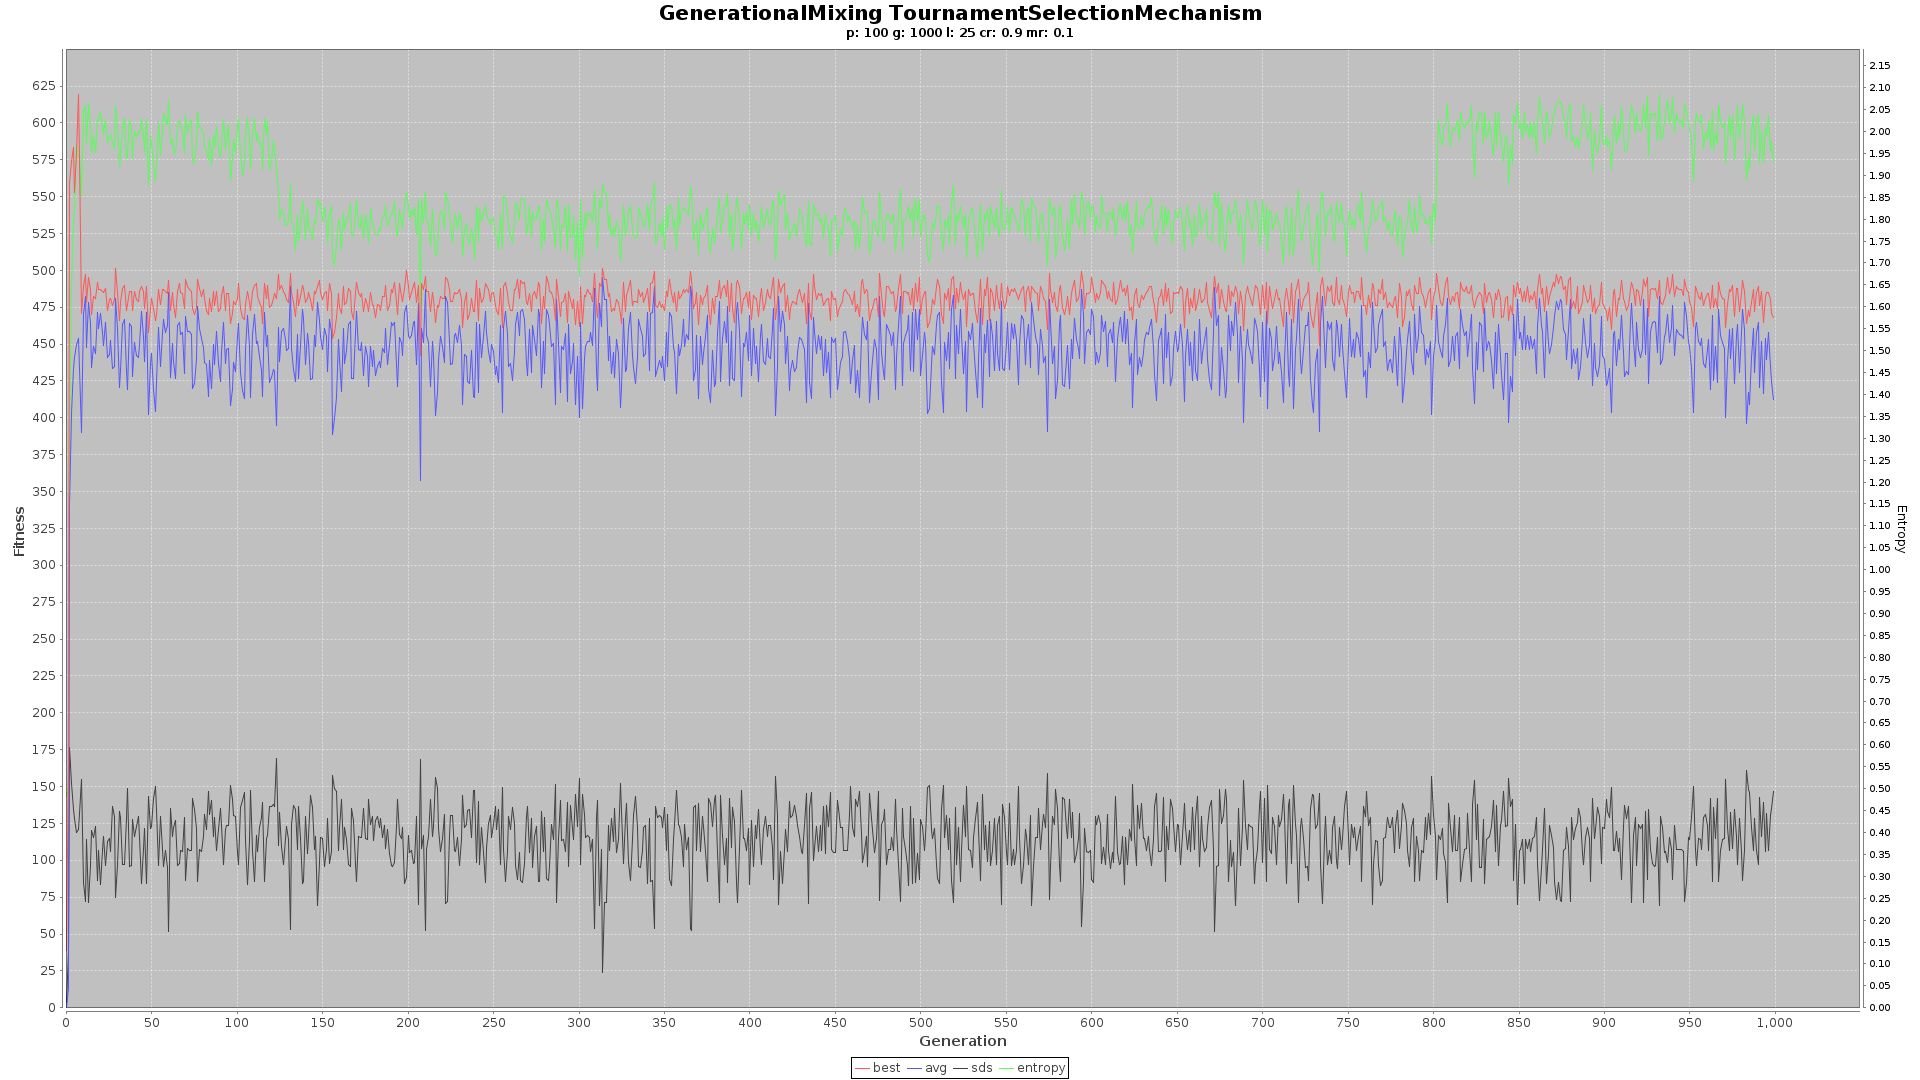
\includegraphics[width=\columnwidth]{b/5/d510.png}%
	\caption{BattleNo.: 5 rf: 1 lf: 0}%
	\label{fig:510}%
	\end{figure}
	Figure \ref{fig:5x1} displays an interesting case where there is a continuous shifting between a lot of strategies, with the exception of the middle. 
	\begin{figure}[H]%
	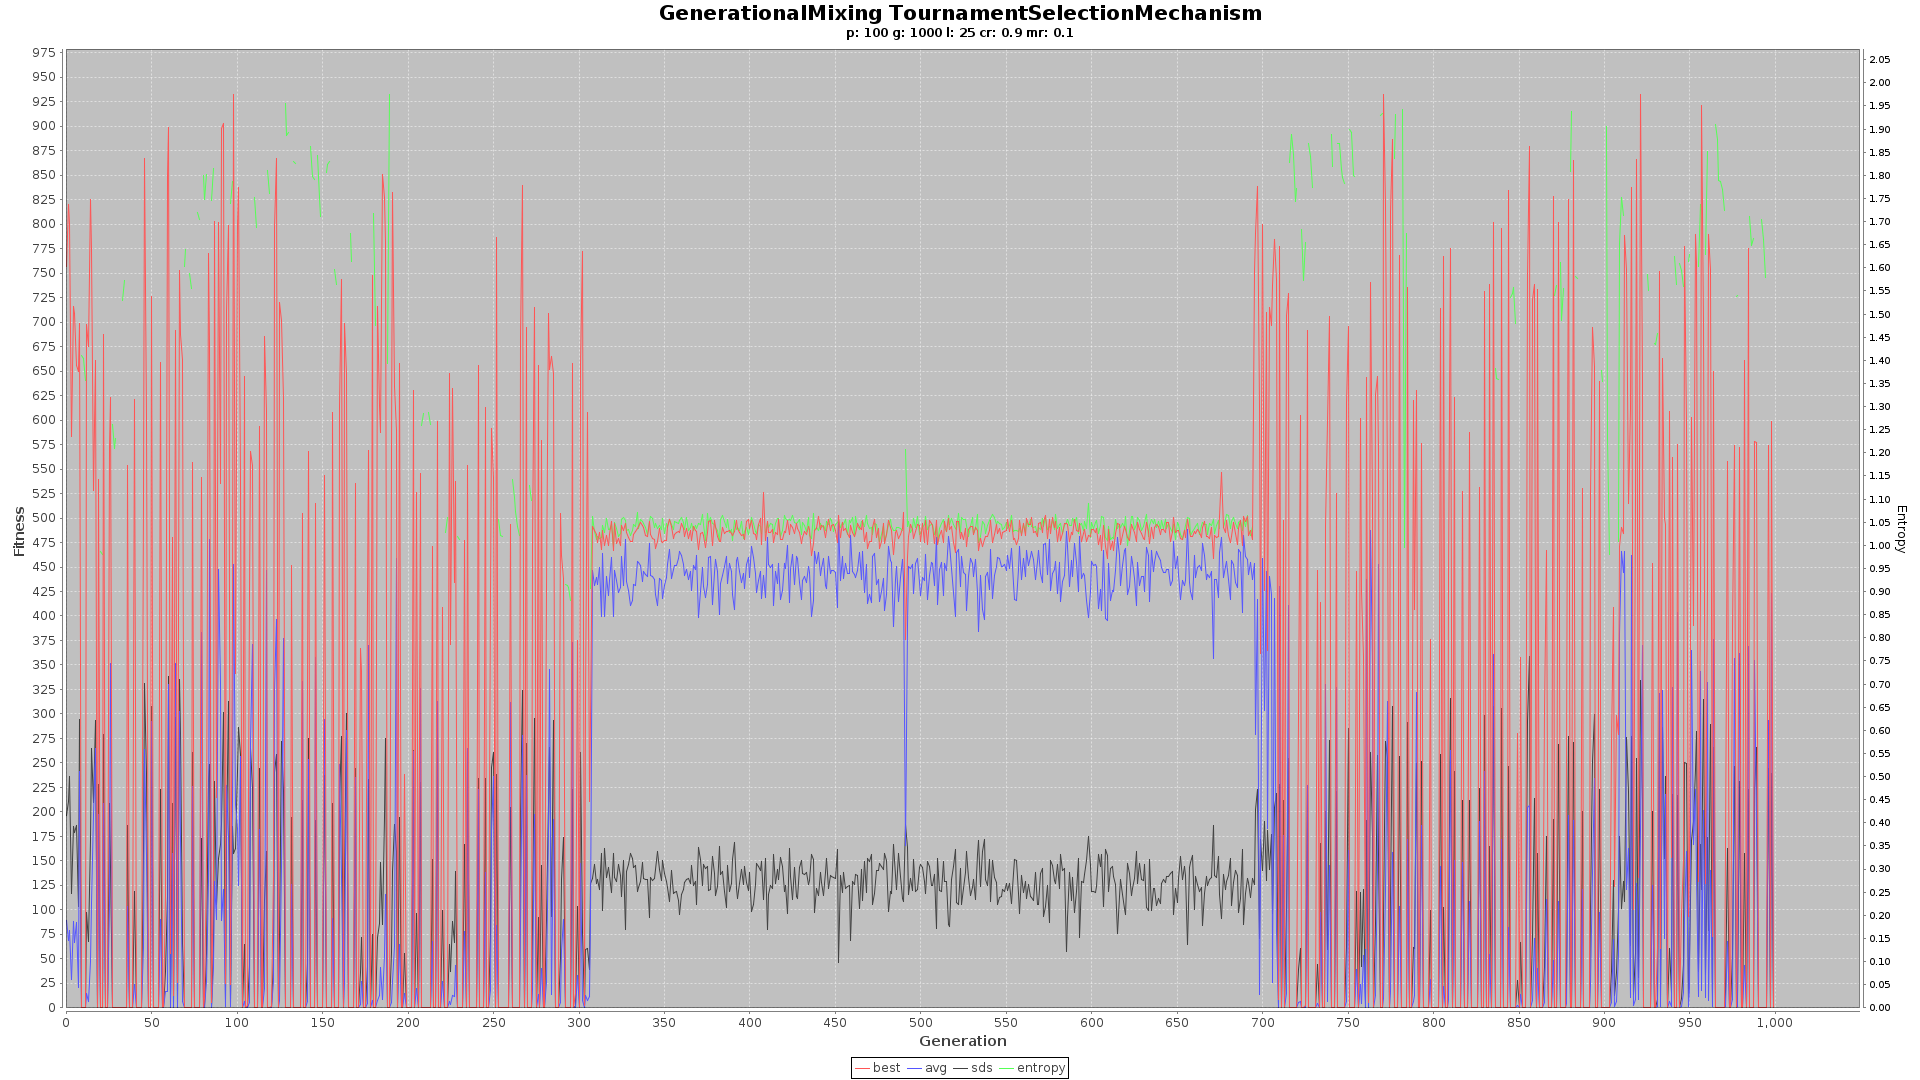
\includegraphics[width=\columnwidth]{b/5/h5x1.png}%
	\caption{BattleNo.: 5 rf: 0.5 lf: 1}%
	\label{fig:5x1}%
	\end{figure}
	Figure \ref{fig:201} shows an example of a convergence to one stable strategy. 
	\begin{figure}[H]%
	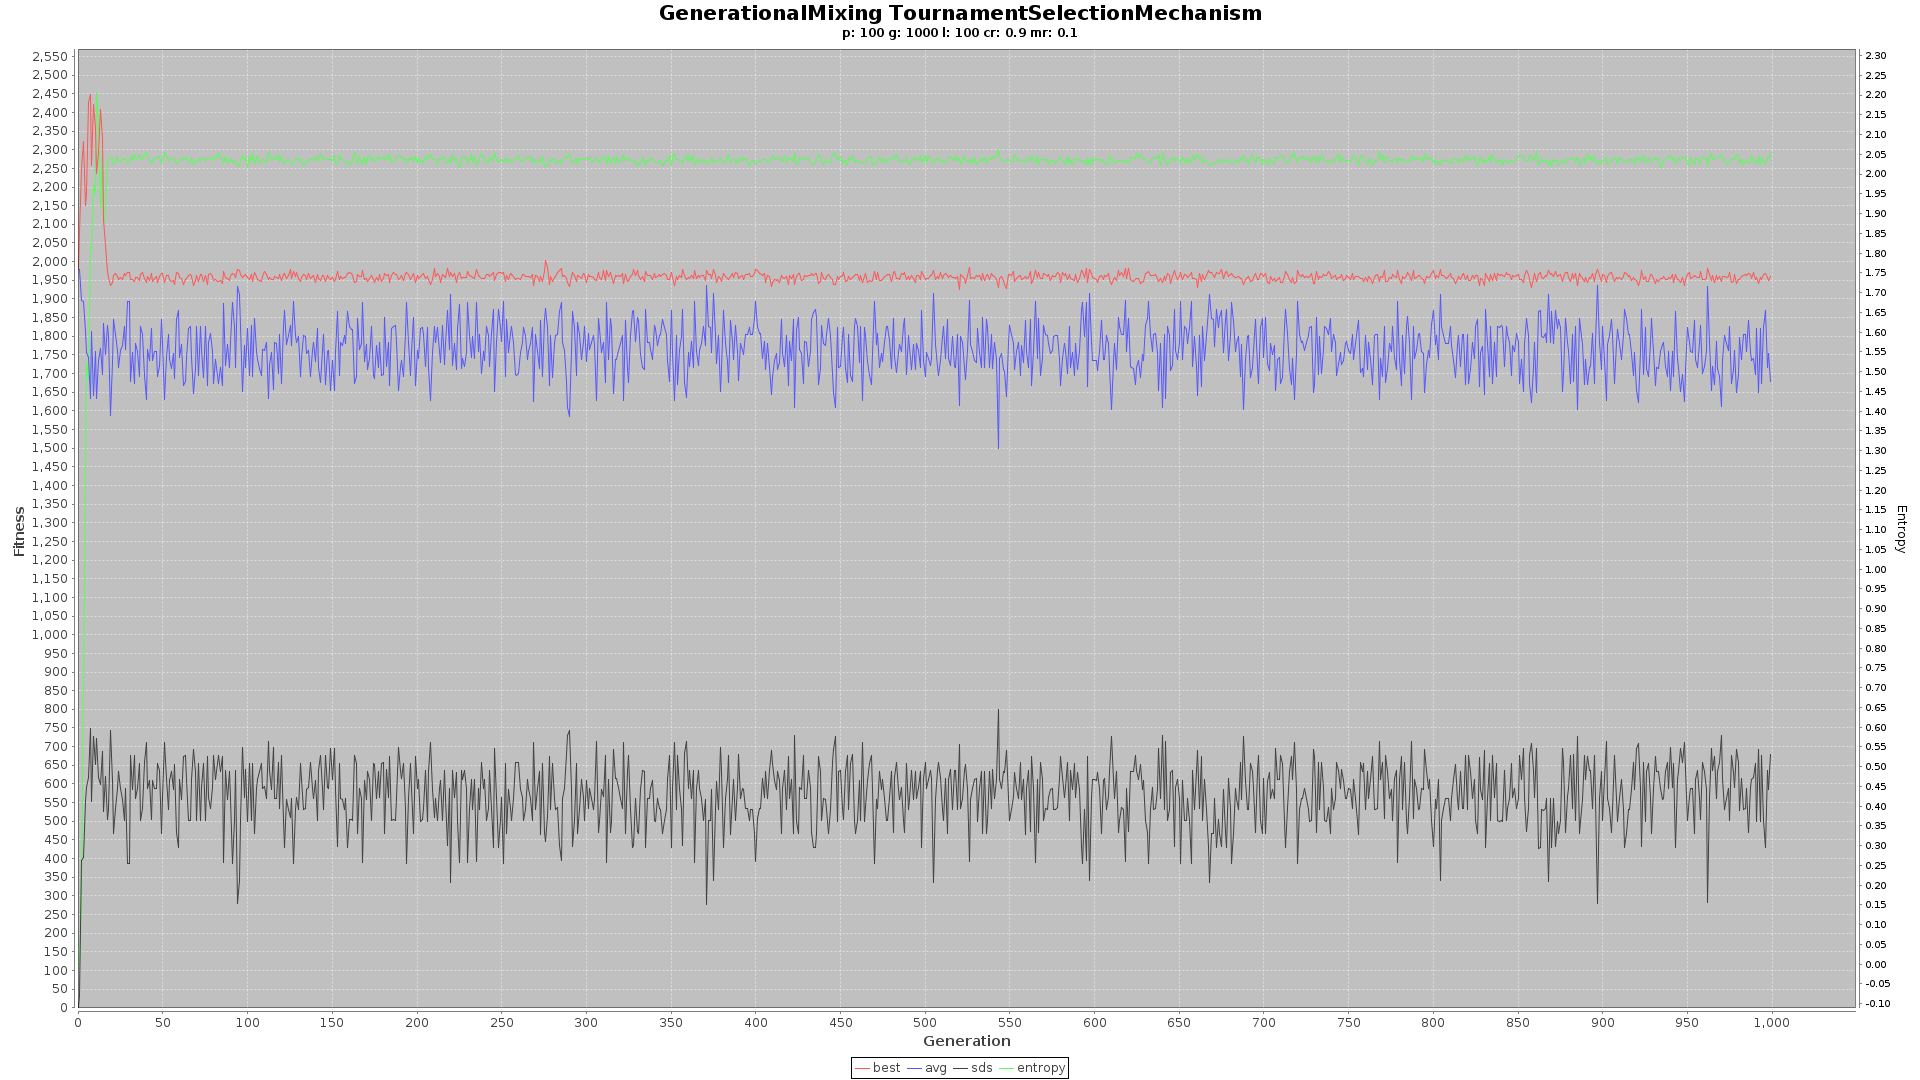
\includegraphics[width=\columnwidth]{b/20/b201.png}%
	\caption{BattleNo.: 20 rf: 0 lf: 1}%
	\label{fig:201}%
	\end{figure}
\subsection{Coevolution}
	One of the distinct differences between coevolution and standard evolution is that fitness is measured against the rest of the population instead of a fixed solution. The result of this is that when one individual of the population increases its fitness, the rest of the population shortly adapts. This leads to the average fitness of the population leveling off.  